\section{\sys in Reliable Networks}
\label{sec:design-reliable}

\begin{figure}[t]
\centering
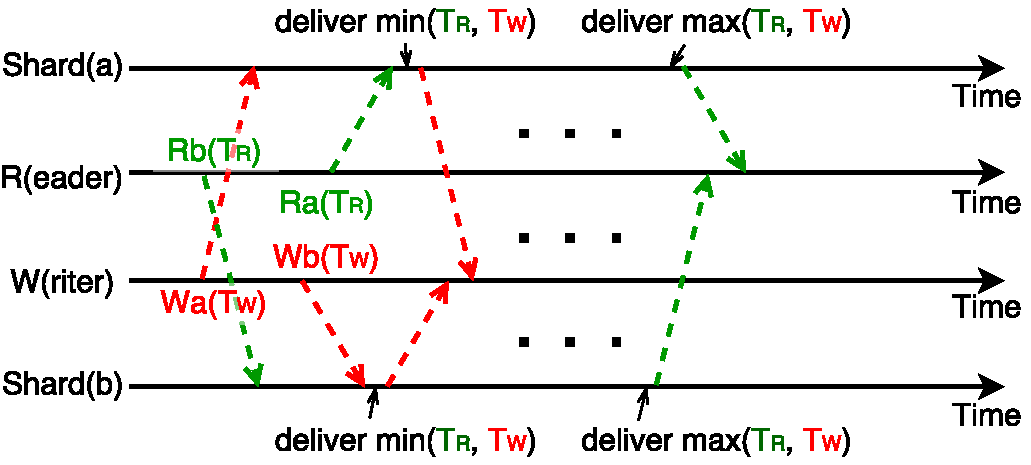
\includegraphics[width=0.48\textwidth]{images/derive_barriers.pdf}
\caption{Deriving barriers with senders $R, W$ and receivers Shard($a$), Shard($b$). Assume $T_W < T_R$.}
\label{fig:barrier}
\vspace{-1em}
\end{figure}

In this section, we assume that all hosts, network switches and links are reliable.
Figure~\ref{fig:barrier} shows an IRIW example where reader $R$ sends $R_a$ and $R_b$ to shard($a$), while writer $W$ sends $W_a$ and $W_b$ to shard($b$).
When shard($a$) receives both $R_a$ and $W_a$, due to monotonic timestamp assignment and the FIFO property between pairs of sender and receiver, shard($a$) knows that it will no longer receive timestamp $T \leq \min(T_R, T_W)$ from either $R$ or $W$, so it can safely process messages with $T \leq \min(T_R, T_W)$.

%\textbf{Scalability}.
%If there are $N$ senders and $N$ receivers, the complexity of communication is $O(N^2)$.
%Sec.\ref{sec:ideal} leverages network switches to merge beacons hierarchically and reduce the beacon message complexity to $O(N)$.

%\textbf{Liveness}.
%If either $R$ or $W$ stops sending messages, shard($a$) can not deliver messages with timestamps higher than $\min(T_R,T_W)$, causing a livelock.
%To ensure liveness, each network link sends \textit{beacon} messages periodically (Sec.\ref{sec:beacon}).

%\textbf{Reordering delay}.
%To minimize \textit{reordering delay}, which is the delay between receiving and delivering a message, Sec.\ref{sec:sync} synchronizes clocks at senders.

%\textbf{Packet loss}.
%If a packet is lost, the receivers will observe an incomplete ordering of events.
%Simple retransmission with same timestamp violates the monotonic property of timestamps.
%The detection and recovery of packet losses are discussed in Sec.\ref{sec:lossy}.

%\textbf{Fault tolerance}.
%Sec.\ref{sec:failure} discusses how to add end hosts, switches and links on the fly, with minimal impact on system performance, and how to merge two existing \sys systems.

%\textbf{Inter-DC topology}.
%Sec.\ref{sec:inter-dc} extends the design to inter-DC topology where routing paths are not loop-free.


\subsection{Hierarchical Merge of Barriers}
\label{sec:ideal}

\begin{figure}[t]
\centering
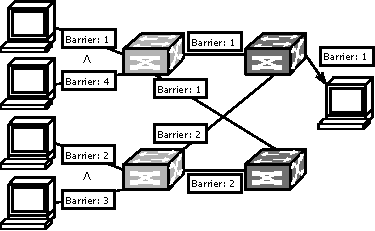
\includegraphics[width=0.4\textwidth]{images/hierarchical_merge.pdf}
\caption{Hierarchical aggregation of timestamp barriers.}
\label{fig:hierarchical_merge}
\vspace{-0.9em}
\end{figure}

In the Lamport-style~\cite{lamport1978time} approach above, with $N$ senders and $N$ receivers, the complexity of communication is $O(N^2)$.
Our solution is to \textit{separate the control plane from the data plane}.
Instead of buffering packets, each network switch only maintains ordering information (aka the control plane), while packets are forwarded as usual (aka the data plane).
We attach two fields to each packet.
The first is a \textit{message timestamp} field, which is only used by end-hosts and won't change once assigned.
The second is a \textit{barrier timestamp} field, which is initialized by end-hosts but will be modified by switches.

%In this case, the control plane is the ordering information, and the data plane is the messages.
%Instead of buffering messages at each network switch, we add a \textit{barrier timestamp} field to each packet.
%Thus, each packet contains two timestamp fields: a \textit{message timestamp} used by end hosts, and a \textit{barrier timestamp} used by both end hosts and switches. 
%At beginning, a packet is formed by an end host which fills the same timestamp value in both fields.
%As the packet moves along the route,  its barrier timestamp is modified by the switches in each link while its message timestamp is unchanged.

The property of the barrier timestamp is:

\emph{When a switch or an end host receives a packet with barrier timestamp $B$ from a network link $L$, it indicates that all future packets from link $L$ will have higher message and barrier timestamps than $B$.}

To derive barriers, senders assign the same value to both fields.
A network switch maintains a register $R_i$ per ingress port $i \in \mathcal{I}$, where $\mathcal{I}$ is the set of all ingress ports.
After routing a packet with barrier timestamp $B$ from ingress port $i$ to the egress port $E$, the switch updates register $R_i := B$, and modifies the barrier timestamp of the packet to a new value $B_{new}$:

%\RED{$i$ never appeared before, while $I$ did. $\exists$ is redundant}
\begin{equation}\label{equ:derive_barriers}
%\RED{
B_{new}:=\min\{R_i| i\in \mathcal{I}_E\}
%}
\end{equation}
%B := \min \{ R_i | \exists i \rightarrow E, i \in \mathcal{I} \}
Where 
\begin{equation}\label{equ:derive_barriers1}
\mathcal{I}_E =\{i| i\rightarrow E, i \in \mathcal{I} \}
\end{equation}

Here $\rightarrow$ means \textit{can be routed to}.
$\mathcal{I}_E$ can be predetermined at route configuration time.
%Note that the switches do not read or modify message timestamps. 
In Appendix~\ref{appx:hierarchical_merge}, we prove that the hierarchical merge described in (\ref{equ:derive_barriers}) and (\ref{equ:derive_barriers1}) maintains the property of barrier timestamps.

When a receiver receives a packet with barrier timestamp $B$, it puts the packet into a priority queue ordered by message timestamps, then delivers all packets with message timestamp below $B$ to the application.

One liveness requirement of the system is \textit{Loop-Free Routing}(Sec.\ref{sec:assumptions}).
%{The liveness of the system is guaranteed if there are no \textit{routing loops} in the network (Sec.\ref{sec:assumptions}).}
If there is a routing loop of links $L_1, \ldots , L_n$, then the barrier timestamps $B_{L_2} \leq B_{L_1}, \ldots, B_{L_n} \leq B_{L_{n-1}}, B_{L_1} \leq B_{L_n}$. So we can't increase the barrier timestamp because a packet may be forwarded in this routing loop indefinitely.
%{, so the barrier timestamps cannot increase.
%This result is evident because a packet may be forwarded in this routing loop indefinitely, therefore we cannot increase the lower bound of in-flight message timestamps.}
When the routing loop is removed, barrier timestamps will start increasing again.

Although the design above works on a P4 programmable switch, many commodity switching chips are not capable of storing states $R_i$ and calculating the minimum among $R_i$.
By using beacon packets as \textit{slacked barriers} of data packets, we can still offload the control plane entirely to the CPU on switches. This will be discussed in Sec.~\ref{sec:commodity}.

\subsection{Beacons on Idle Links}
\label{sec:beacon}

The liveness of the system requires information from every network link. The receiver cannot distinguish between an idle link or excessive delay on the link. We send periodic \textit{beacons} to ensure the link is always busy.
%There are two ways: (1) let the sender send a signal packet to shutdown the link temporarily; (2) ensure the link is always busy by sending periodic \textit{beacons}.

%The first solution requires the sender to rejoin the receiver when it has another packet to send, which requires at least a single-hop RTT to re-sync the timestamps (Sec.\ref{sec:failure}). Therefore, this solution is applicable when the sender knows it would not send any packet during a relatively long period, \textit{e.g.}, when the application closes.

Beacons not only introduce network and CPU overhead, but also affects reordering delay. The receiver of an idle link can only increase its barrier timestamp every time it receives a beacon. We further synchronize beacons at different network links, so that reordering delay overhead is the beacon interval regardless of number of hops in network path. To this end, we introduce two beacon intervals $B_{min}$ and $B_{max}$. A switch broadcasts beacons as soon as it receives a beacon and have not sent beacons for at least $B_{min}$ time. A switch also broadcasts beacons when it has not received a beacon for $B_{max}$ time. $B_{min}$ is set to the estimated maximum path delay variance, while $B_{max}$ is the desired beacon interval. The network/CPU overhead and reordering delay is a trade-off to choose $B_{max}$.

When a sender is idle for a timeout significantly longer than RTT, it notifies the switch and stops sending beacons. When it sends messages via \sys again, it can rejoin within an RTT (Sec.\ref{sec:failure}).

\iffalse
%Remove the algorithm because it does not contain much information and takes too much space.
\setlength{\textfloatsep}{1em}
\begin{algorithm}[t]
 \DontPrintSemicolon
 \textbf{Parameters:} beacon intervals $min$, $max$\;
 \textbf{States:} Ingress port barrier timestamp $R_i, i \in \mathcal{I}$\;
   \qquad Egress port barrier timestamp $B_e, e \in \mathcal{E}$\;
   \qquad Last sent barrier time last$_e, e \in \mathcal{E}$\;
   \qquad Local physical clock, fetched via \textit{time()}\;
   \qquad timer$_e, e \in \mathcal{E}$ that fires after a given interval\;
 \SetKwProg{Fn}{Function}{ begin}{end}
 \SetKwFunction{SendBeacon}{SendBeacon}
 \Fn{\SendBeacon{\textnormal{barrier} $B_E$, \textnormal{egress port} $E$}}{
    Send beacon packet $B_E$ to $E$\;
    last$_E \leftarrow$ time()\;
    reset timer$_E$ to fire after $max$\;
 }
 \SetKwFunction{UpdateEgressPortTS}{UpdateEgressPortTS}
 \Fn{\UpdateEgressPortTS{\textnormal{egress port} $E$}}{
    $B_E \leftarrow \min \{ R_i | i \rightarrow E, i \in \mathcal{I} \}$\;
    \eIf{last$_E + min \leq$ time()}{
      SendBeacon ($B_E$, $E$)\;
    }{
      reset timer$_E$ to fire after last$_E + min - $time()\;
    }
 }
 \textbf{Event processing:}\\
 \If{receive a beacon or data packet $P$}{
  read barrier timestamp $b$ from packet $P$\;
  $R_I \leftarrow b$, where $I$ is the ingress port of $P$\;
  \If{$P$ is a data packet}{
  	determine egress port $E$ of $P$ by routing\;
    UpdateEgressPortTS ($E$)\;
    modify barrier timestamp in $P$ to $B_E$\;
  }
  \ElseIf{$P$ is a beacon packet}{
  	\ForEach{$e \in \{ e \in \mathcal{E} | I \rightarrow e \}$}{
    	UpdateEgressPortTS ($e$)\;
    }
  }
 }
 \ElseIf{timer$_E, E \in \mathcal{E}$ fires}{
    SendBeacon ($B_E$, $E$)\;
 }
 \caption{Timestamp processing with beacons.}
 \label{alg:beacon}
\end{algorithm}
\fi

%In order to detect failures, each switch has a timeout timer per ingress port. If no beacon or data packet is received for three max beacon intervals, the ingress port is considered to be dead and removed from the ingress port list. When the failed link, host or switch recovers, it needs to rejoin (Sec.\ref{sec:incremental}).

\subsection{Minimax Clock Synchronization}
\label{sec:sync}

%\RED{\sout{People perceive two events as simultaneous when observing their effects at the same time.}}
%Due to different propagation delays from the origin of events to the observers, simultaneity of events is relative to observers.
%From an end-host receiver's perspective, two events should be simultaneous if the messages originated from the events arrive at the receiver simultaneously.
%In a distributed system, events are timestamped and their effects propagate in the form of packets.
%On one hand, we hope to timestamp the events so that if two packets originated from two distant events arrive at a receiver simultaneously, these two events should have a same timestamp.
%On the other hand, unlike our physical universe, a distributed system is easier to reason if the ordering of events is globally consistent, \textit{i.e.}, all receivers agree on the timestamps of events.

The next challenge is how to assign timestamps to messages.
Clock synchronization in data centers becomes increasingly accurate leveraging NIC timestamps~\cite{correll2005design}, GPS~\cite{corbett2013spanner}, PHY~\cite{lee2016globally} and network effects~\cite{geng2018exploiting}. However, delay variance of network paths makes physical time a suboptimal choice for timestamps.
Different OS network stacks have more than 100~$\mu$s of processing delay differences, and it may increase to milliseconds under heavy load.
Links with different speeds or congestions also lead to delay variations.
For example, two messages are transmitted from two senders to the same receiver at the same physical time. However, they arrive at different times due to different network delays. As a result, the earlier one must wait for the later one to be processed together, which increases reordering delay.

To this end, we devise a new algorithm to synchronize logical clocks on senders and assign message timestamps according to the clocks. We begin with a simplistic case with multiple senders $S_i \in \mathcal{S}$ and one receiver $R$. Assume the one-way network delays are $d_i$ for $S_i \rightarrow R$ and $r_i$ for $R \rightarrow S_i$. Note that we can measure the round-trip time ($RTT_i = d_i + r_i$) between two nodes, but one-way delay is hard to measure. We further observe that speed of clocks on each node have negligible difference (relative error less than $10^{-5}$~\cite{corbett2013spanner,geng2018exploiting}), while in the long run they will diverge. We consider physical clocks precise enough to measure short intervals.

To minimize reordering delay, we want the senders to assign timestamps so that messages with a same timestamp arrive at receiver simultaneously. Consequently, the logical clock at $S_i$ should have an offset $d_i$ to the physical time. If $R$ broadcasts a clock synchronization message at physical time 0, $S_i$ will receive it at $r_i$. Then $S_i$ compensates a round-trip time $RTT_i$ to the received timestamp and sets its clock to $0 + d_i + r_i$ at physical time $r_i$, which has offset $d_i$ to physical time. Our goal is achieved.


\begin{algorithm}[t]
 \DontPrintSemicolon
 \textbf{States:} Clock adjustment offset $off$\;
 \qquad Last assigned timestamp $T_{last}$\;
 \qquad Local physical clock, fetched via $time()$\;
 \textbf{Event processing:}\;
 \If{received sync timestamp $T_{sync}$}{
 	$off \leftarrow T_{sync} - time()$\;
 }
 \ElseIf{a total-ordered event occurs}{
    TS $\leftarrow \max (T_{last} + 1, time() + off)$\;
    $T_{last} \leftarrow$ TS\;
 }
 \caption{Clock adjustment and timestamp assignment on each end host.}
 \label{alg:clock}
\end{algorithm}



Because timestamps can only increase monotonically, when the newly synchronized offset $d_i$ is less than the current offset of $S_i$, it has to ``stall'' the logical clock rather than decreasing it. During stall, the logical clock increments by 1 per scattering, while the synchronized offset increases at the speed of physical clock. Algorithm~\ref{alg:clock} shows the procedure.

Now we extend to multiple receivers $R_i \in \mathcal{R}$.
%In a data center, each sender is also a receiver, but we denote the send and receive roles separately for clarity.
Assume the one-way delays are $d_{ij}$ for $S_i \rightarrow R_j$ and $r_{ij}$ for $R_j \rightarrow S_i$, and we can measure $RTT_{ij} = d_{ij} + r_{ij}$. If we want to follow the approach above for each receiver, we need to synchronize the clocks of receivers first. In this regard, we add a \textit{forward pass} in which $S_i$ send to $R_j$ and synchronize clocks of $R_j$, then run the \textit{backward pass} above from $R_j$ to $S_i$. In both forward pass and backward pass, each node receives potentially different offsets from multiple peers, so we need two aggregation functions to resolve conflicts, namely \texttt{FwdFunc} and \texttt{BackFunc}. Assume the sender logical clocks are $T_k, k \in \mathcal{S}$ initially, the new logical clocks $T'_k$ should be:

\vspace{-1em}
\begin{equation*}
\begin{aligned}
T'_k & = \texttt{BackFunc} \{ \texttt{FwdFunc} \{ T_i - d_{ij} \} - r_{jk} + RTT_{kj} \} \\
     & = \texttt{BackFunc} \{ \texttt{FwdFunc} \{ T_i - d_{ij} \} + d_{kj} \}
\end{aligned}
\end{equation*}

Because a logical clock needs to be stalled if it is synchronized to a lower offset, and the reordering delay during stall is not optimal, we aim to minimize clock stall. Consequently, all clocks should catch up with the clock with highest offset, indicating that \texttt{FwdFunc} should be \texttt{max}. If we choose \texttt{BackFunc} to also be \texttt{max}, in some networks with delay imbalance, the clocks would not converge. Convergence means that $\forall k \in \mathcal{S}, T'_k = T_k$. In this regard, we choose \texttt{BackFunc} to be \texttt{min}. Appendix~\ref{appx:minimax} proves that given any initial clock offsets, clocks converge in one RTT. This ensures self-stabilization in a network with rapidly changing delays.


\begin{figure*}[t]
\centering
	\subfloat[Forward aggregation (max).\label{fig:minimax_max}]
	{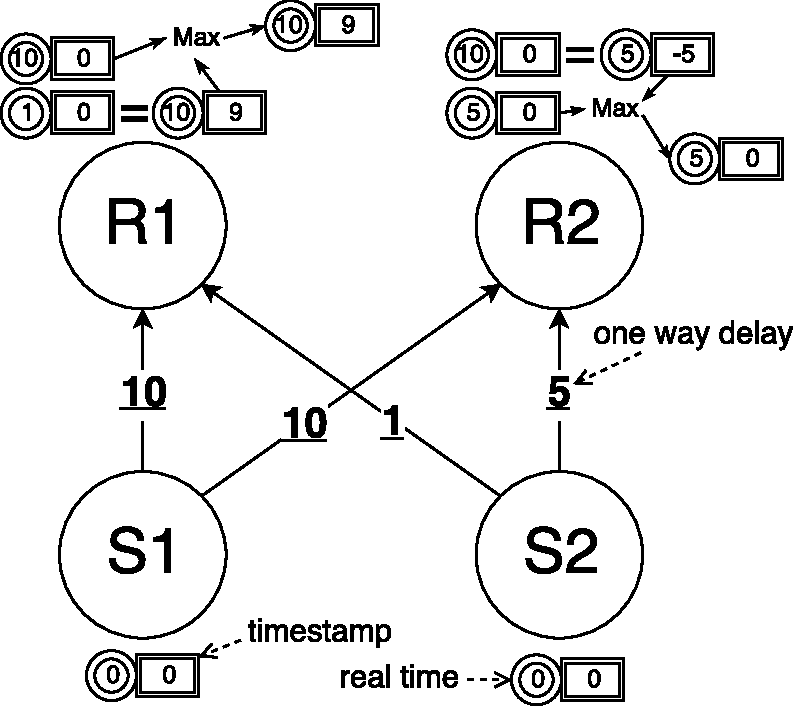
\includegraphics[width=.33\textwidth]{images/minimax_example_1.pdf}}
	%\hspace{0.08\textwidth}
	\subfloat[Backward aggregation (min) and RTT compensation.\label{fig:minimax_min}]
	{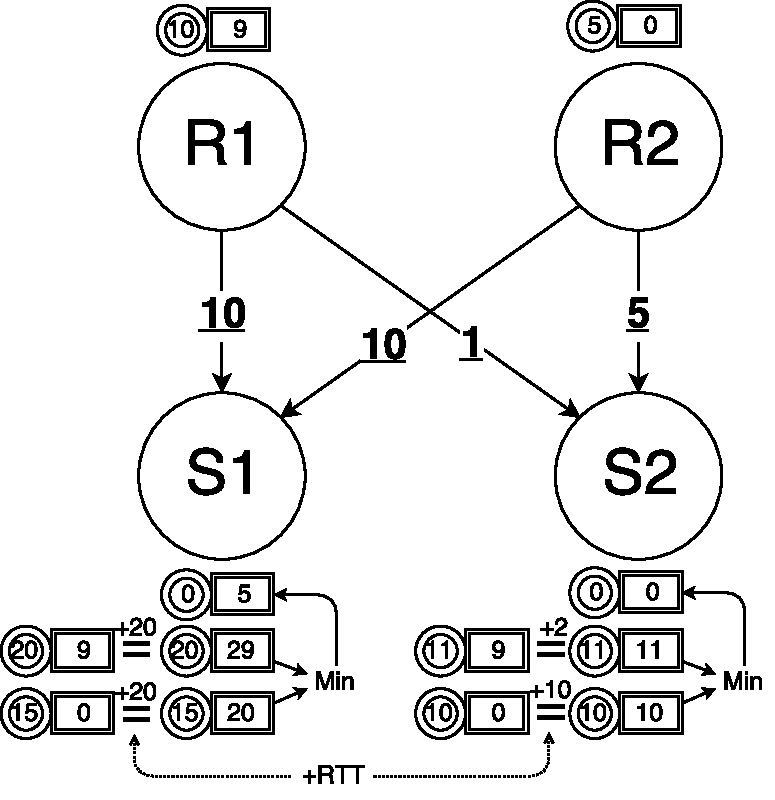
\includegraphics[width=.33\textwidth]{images/minimax_example_2.pdf}}
	%\hspace{0.08\textwidth}
	\subfloat[Reorder delay after synchronization.\label{fig:minimax_result}]
	{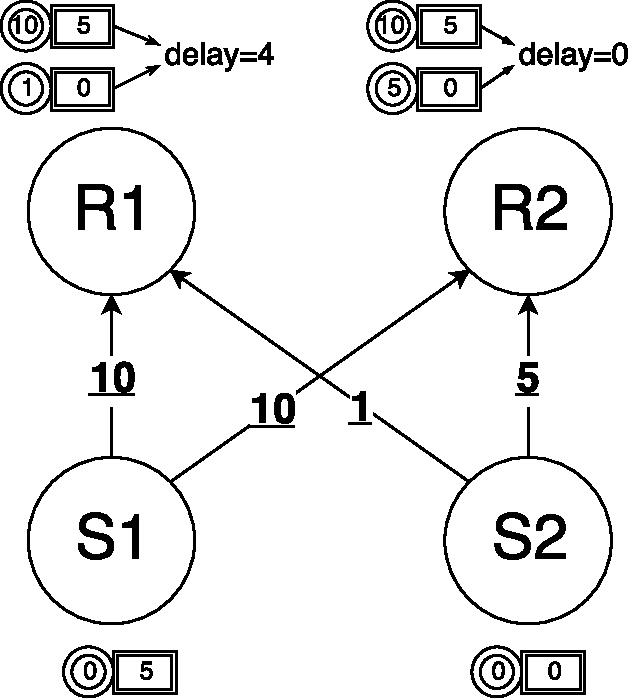
\includegraphics[width=.3\textwidth]{images/minimax_example_3.pdf}}

\caption{Illustration of minimax clock synchronization.}
\label{fig:minimax}
\vspace{-1.2em}
\end{figure*}



Fig.~\ref{fig:minimax} shows an example with two senders and two receivers.
In Fig.~\ref{fig:minimax_max}, each receiver chooses the maximum timestamp offset from physical clock and broadcasts the offset back to sender. Initial reordering delays are 10 at $R_1$ and 5 at $R_2$.
In Fig.~\ref{fig:minimax_min}, each sender adds RTT to received offsets and synchronizes to the minimum offset.
Fig.~\ref{fig:minimax_result} shows that after minimax synchronization, reordering delays reduce to 4 at $R_1$ and 0 at $R_2$.

Without in-network computation, clock synchronization would require $O(N^2)$ messages. Similar to hierarchical aggregation of barriers, we use network switches to aggregate \texttt{min} and \texttt{max} timestamps hierarchically, as shown in Algorithm~\ref{alg:minimax}.

\iffalse
The first property is necessary for correctness. The second property ensures numerical stability, \textit{i.e.}, the increase speed of timestamps does not vanish or explode. In addition, the second property enables us to obtain an unbiased estimate of the event timestamp after one round trip, by measuring RTT with a local physical clock. The third property minimizes reordering delay by optimizing for simultaneous arrival of a message timestamp and its corresponding barrier timestamp.

To maintain the second property, we store event timestamps as \textit{offsets} relative to local physical clock on end hosts and switches. When sending timestamps to the network, we add current clock time back to the offset.
This effectively uses physical clock to measure \textit{relative time} instead of absolute time, so the clock skew would not accumulate. Physical clocks driven by crystal oscillators and CPU instruction counters are accurate enough to measure short intervals, because their relative error is less than $10^{-5}$~\cite{corbett2013spanner} and the granularity is at nanosecond level to ensure each packet has a unique timestamp.
It worth noting that Sec.~\ref{sec:ideal} stores a timestamp barrier as an \textit{absolute value} to represent a slacked bound, while this subsection stores event timestamps as \textit{relative offsets} to represent unbiased estimations.

For the third property, we determine new event timestamp on end hosts according to feedback information from the network.
The synchronized timestamp from the network may be smaller than the last assigned event timestamp $T_{last}$. To prevent the event timestamps from decreasing, we track $T_{last}$ and let the new event timestamp to be the maximum of $T_{last} + 1$ and synchronized timestamp, as shown in Algorithm~\ref{alg:clock}. This effectively ``stalls'' the event timestamp until the synchronized timestamp catches up with it.
\fi


\iffalse
To derive the timestamp feedback in the network, we need to estimate the delay from end-host senders to end-host receivers.
One-way delay is hard to measure, therefore we use round-trip time (RTT) instead.
Each end-host will add RTT to received feedback timestamp, just as illustrated in Figure~\ref{fig:minimax_min}.
When considering switches, one-hop RTT will be measured and compensated for feedback by each switch.

The challenge is that there are multiple senders and receivers, so we must aggregate timestamps from different hosts.
Let \texttt{FwdFunc} aggregate sender timestamps $T_i, i \in \mathcal{S}$ and \texttt{BackFunc} aggregate feedbacks from receivers $j \in \mathcal{R}$.
To simplify discussion, assume $d_{ij}$ is a fixed (but not measurable) one-way delay from sender $i$ to a receiver $j$, $r_{ji}$ is the fixed delay from receiver $j$ to sender $i$, and $RTT_{ij} = d_{ij} + r_{ji}$ is measurable. The new event timestamp $T'_k$ on a sender $k \in \mathcal{S}$ is:

\begin{equation*}
\begin{aligned}
T'_k & = \texttt{BackFunc} \{ \texttt{FwdFunc} \{ T_i - d_{ij} \} - r_{jk} + RTT_{kj} \} \\
     & = \texttt{BackFunc} \{ \texttt{FwdFunc} \{ T_i - d_{ij} \} + d_{kj} \}
\end{aligned}
\end{equation*}

On one hand, because timestamps must grow monotonically, all clocks in the system should catch up with the clock with highest timestamp.
To this end, $T'_k$ needs to reflect the maximum of sender timestamps $T_i$. Because $T_i, \forall i$ only appears in \texttt{FwdFunc}, \texttt{FwdFunc} needs to be $max$.

On the other hand, to ensure the second and fourth property of event timestamps, $\Sigma T_k, \forall k$ should converge. Choosing \texttt{BackFunc} as $min$ and \texttt{FwdFunc} as $max$ guarantees that each timestamp converge after one RTT for any initial assignment of $T_k$, \textit{i.e.}, $\forall k, T'_k = T''_k$. This self-stabilization property is proved in Appendix \ref{appx:minimax}.

Figure~\ref{fig:minimax} is a simple example of minimax synchronization.
The network consists of only two senders and two receivers.
In Figure~\ref{fig:minimax_max}, both senders assign timestamp to $0$ at the very beginning (equivalent to physical clock synchronized).
Based on linear time assumption, both receivers choose the maximum timestamp as feedback.
In Figure~\ref{fig:minimax_min}, both senders add RTT to feedback and synchronize to the minimum feedback timestamp.
Figure~\ref{fig:minimax_result} shows that compared to the original timestamp assignment, reorder delay declines after minimax synchronization.

Finally, to reduce the message complexity of clock synchronization, we use network switches to aggregate the $min$ and $max$ timestamps hierarchically, as shown in Algorithm~\ref{alg:minimax}.
\fi

\setlength{\textfloatsep}{0em}
\begin{algorithm}[t]
 \DontPrintSemicolon
 \textbf{States:} Per-port max timestamp $max_i, i \in \mathcal{I}$\;
 	\qquad Per-port min timestamp feedback $min_e, e \in \mathcal{E}$\;
    \qquad RTT estimation per egress link, $RTT_e, e \in \mathcal{E}$\;
    \qquad Received RTT probe request, $rttreq_i, i \in \mathcal{I}$\;
 	\qquad Local physical clock, fetched via $time()$\;
 \textbf{Event processing:}\\
 \If{send beacon packet to port $P$}{
    piggyback the following with the beacon packet:\\
 	max timestamp $T_{max}$:\\
    \quad $T_{max} = \max \{ max_i | i \in \mathcal{I} \wedge i \rightarrow P \} + time()$\;
    min timestamp $T_{min}$:\\
    \eIf{$\exists e, e \in \mathcal{E} \wedge P \rightarrow e$} {
        $T_{min} = \min \{ min_e | e \in \mathcal{E} \wedge P \rightarrow e \} + time()$\;
    }{
    	$T_{min} = T_{max}$\;
    }
    RTT probe request $rtt_{req}$:\\
    \quad $rtt_{req} = time()$\;
    RTT probe response $rtt_{ack}$:\\
    \quad $rtt_{ack} = time() - rttreq_P$\;
 }
 \ElseIf{received beacon packet from port $P$}{
    extract $T_{max}, T_{min}, rtt_{req}, rtt_{ack}$ from beacon\;
    $RTT_P \leftarrow \alpha \cdot (time() - rtt_{ack}) + (1 - \alpha) \cdot RTT_P$\;
 	$max_P \leftarrow T_{max} - time()$\;
    $min_P \leftarrow T_{min} + RTT_P - time()$\;
    $rttreq_P \leftarrow time() - rtt_{req}$\;
 }
 \caption{Minimax clock synchronization on each network switch and end host (treated as a single-port switch).}
 \label{alg:minimax}
\end{algorithm}


%One may ask why we use physical clock instead of Lamport clock (cite) or vector clock (cite) to measure intervals. A clock measures an interval by counting repetitive events. A good clock source should generate a roughly same number of repetitive events when our measurement object is stable, as well have a granularity finer than the intervals to measure.
%If we use packet counter as clock source, the RTT measurement will vary with network throughput. If we use received timestamps as clock source, it is unable to measure a tiny interval if no packet is received during the interval. Physical clocks driven by crystal oscillators and CPU instruction counters are accurate enough to measure short intervals, because their relative error is less than $10^{-5}$ (cite) and the granularity is as fine as a nanosecond.



\section{\sys in Unreliable Networks}
\label{sec:reliable}

Previous section achieves TOMS in reliable networks. In this section, we discuss how to maintain the ordering and atomicity of message delivery in the presence of packet losses, packet corruptions and node failures.

\subsection{Packet Loss Detection and Recovery}
\label{sec:lossy}

In data centers, network links experience one packet loss or corruption every $10^5$ \texttildelow $10^7$ packets~\cite{zhuo2017understanding}.
Additionally, some devices or network links may have congestion or bugs that lead to higher packet loss possibility~\cite{guo2015pingmesh}.
%\sys detects packet loss in the network and mark barrier timestamps with a \textit{loss encountered} flag.
\sys detects packet loss in the network using per-port packet loss counter in commodity NICs and switches. Because switches do not have enough buffer~\cite{bai2017congestion}, we rely on end hosts to locate and retransmit lost packets via TCP-like loss recovery.

Our aim is to deliver messages in an one-way network delay when no packet loss encountered, and fall back to two-phase commit (2PC) with three one-way delays when loss occurs. For this purpose, we rename the original barrier to \textit{unreliable barrier} and add a \textit{commit barrier} and a \textit{loss encountered} flag alongside it. Commit barrier carries accumulative commit timestamp from the sender, which means that all messages sent by the sender and below commit timestamp has been received. Figure~\ref{fig:ack-barrier} shows an example. When loss encountered flag is off, a receiver can deliver messages according to unreliable barrier. Otherwise, it delivers based on commit barrier.


\setlength{\textfloatsep}{1em}
\begin{algorithm}[t]
 \DontPrintSemicolon
 \textbf{States:} Unreliable barrier $UB_i, i \in \mathcal{I}$\;
 	\qquad Commit barrier $CB_i, i \in \mathcal{I}$\;
    \qquad Received loss encountered flag $RLE_i, i \in \mathcal{I}$\;
 	\qquad Last-hop loss encountered flag $LE_i, i \in \mathcal{I}$\;
    \qquad Unreliable barrier at last loss $LB_i, i \in \mathcal{I}$\;
    \qquad Last loss counter $LC_i, i \in \mathcal{I}$\;
    \qquad Current loss counter, fetched via $C(i), i \in \mathcal{I}$\;
 \textbf{Event processing:}\\
 \If{\textnormal{Receive beacon packet from ingress $i$}}{
 	$RLE_i \leftarrow$ loss encounter flag in the packet\;
    $UB_i \leftarrow$ unreliable barrier in the packet\;
    $CB_i \leftarrow$ commit barrier in the packet\;
    \If{$LC_i \neq C(i)$}{
    	$LE_i \leftarrow \textnormal{True}$\;
        $LB_i \leftarrow UB_i$\;
        $LC_i \leftarrow C(i)$\;
    }
	\ElseIf{$CB_i \geq LB_i$}{
    	$LE_i \leftarrow \textnormal{False}$\;
    }
 }
 \ElseIf{\textnormal{Send beacon packet to egress $E$}}{
    Unreliable barrier $\leftarrow \min \{ UB_i | i \in \mathcal{I} \wedge i \rightarrow E \}$\;
    Commit barrier $\leftarrow \min \{ CB_i | i \in \mathcal{I} \wedge i \rightarrow E \}$\;
    Loss encountered flag $\leftarrow \exists i \in \mathcal{I} \wedge (i \rightarrow E) \wedge (LE_i \vee RLE_i)$\;
 }
 \caption{Hop-by-hop loss detection in network switches.}
 \label{alg:loss-detection}
\end{algorithm}

%To detect packet loss in the network, we leverage per-port packet loss counter in commodity NICs and switches.
%If packet loss counter of an ingress port changes, we know that a packet is lost during current interval and set the \textit{loss encountered} flag of the ingress port.
%As a justification, our actual measurements find that the number of end-to-end packet losses agree with the packet drop counters in our test environment.


\begin{figure}[t]
\centering
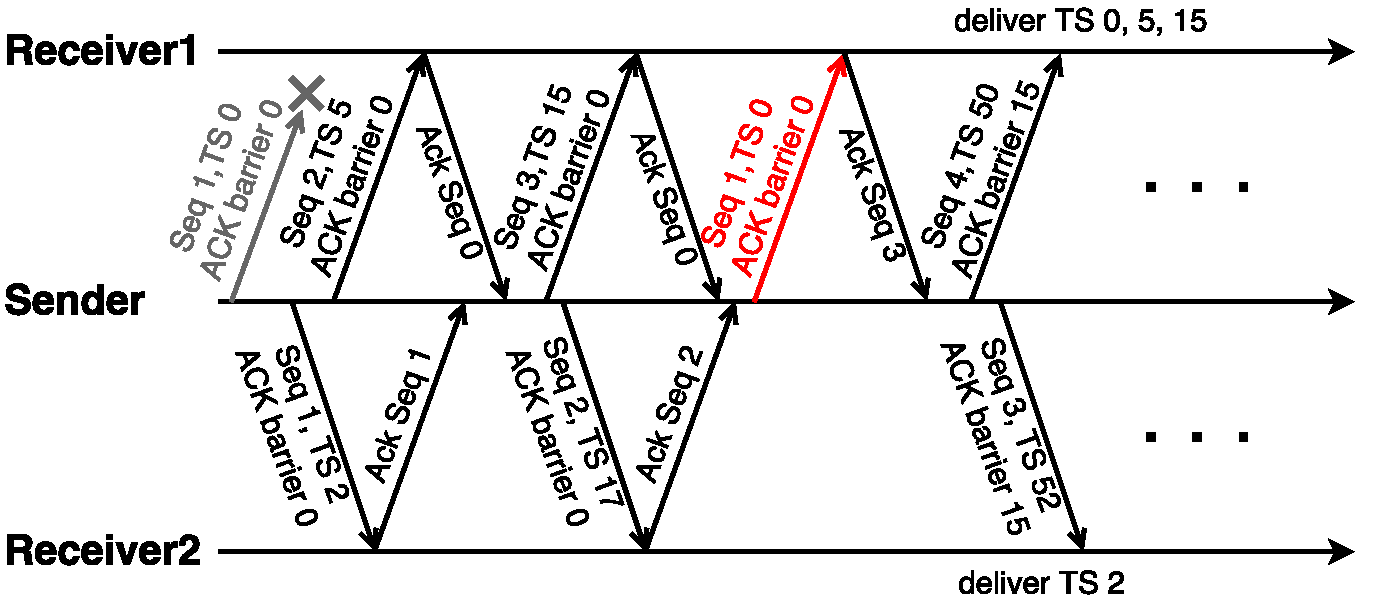
\includegraphics[width=0.45\textwidth]{images/loss_detection.pdf}
\caption{Loss recovery and commit barriers.}
\label{fig:ack-barrier}
\vspace{-0.4em}
\end{figure}



%Similar to TCP, packets have sequence numbers independent of timestamps.
%The receiver responds ACK to the sender via non-timestamped packets.
%For each connection, the sender maintains a \textit{minimum unacknowledged timestamp}, detect packet loss via duplicate ACKs or timeout, then retransmit the lost packets with the same timestamp (Figure~\ref{fig:ack-barrier}).
%Each sender maintains an unacknowledged timestamp barrier (\textit{ACK barrier}), which is the minimum of minimum unacknowledged timestamps among all connections. Messages with timestamps below the ACK barrier are guaranteed to be received by all recipients.

Different from traditional 2PC where commit messages are sent to receivers directly, \sys aggregates commit barriers hierarchically in network. The first reason is that \sys can only deliver a message after all messages with lower timestamps. The second reason is to \textit{clear} the loss encountered flag. As shown in Algorithm~\ref{alg:loss-detection}, when commit barrier is higher than unreliable barrier recorded at last packet loss, the switch clears the flag because messages below commit barrier have been received and messages above that have not been lost.


\subsection{Fault Tolerance and Incremental Deployment}
\label{sec:failure}

Previous section retransmits lost packets with end hosts. When a host, switch or network link fails, we cannot stall the network and wait for it to recover. First, we deal with host failure. When a host fails, the nearby switch will detect it via beacon timeout and broadcast the failure in beacon packets. A receiver discards messages from the failed node in reordering buffer. To ensure message scattering atomicity, a sender checks uncommitted messages and send \textit{recall} messages to other receivers. Upon receiving \textit{recall}, it discards the message in reordering buffer and responds ACK. The sender then discards the uncommitted message when all healthy receivers have recalled. We admit that \sys shares a same limitation with standard two-phase commit. If a receiver fails after commit message has been sent, \sys cannot recall committed messages from other receivers.

When a host recovers from failure, it needs to join \sys system as a new host. Recovering lost messages during failure requires persistence or replication, which incurs high cost and the best choice should be determined by applications rather than \sys transport.

Next, we deal with failure of network switches or links. If a failure does not block communication between any pair of hosts, it only causes a brief interval of packet losses. Otherwise, the sender would timeout in retransmission and \textit{recall} messages from other receivers. If a failure disconnects an end host from the network (\textit{e.g.} ToR switch failure), nearby switches would broadcast the host failure. In the extreme case of network partition, all cross-partition scatterings will fail and scatterings within a partition still proceed with total order.

%Switches and end hosts detect network link or neighbor node failure when no beacons are received within a timeout interval.
%Upon detection of failure, it will install a firewall rule to block data packets from the corresponding port and excludes the port from barrier aggregation and clock synchronization.
%As an effect, the barriers are temporarily stalled during the timeout interval, and proceed to increase after the failure port is excluded.
%In terms of CAP theorem~\cite{brewer2000towards}, we choose availability and partition tolerance over consistency between the partitions.
%When the link or neighbor node recovers, it needs to rejoin the \sys system like a newcomer.

%When an end host or switch needs to join a \sys system, it first initializes a \sys system by itself (all the timestamps are initialized arbitrarily). Therefore, the joining process is reduced to connecting two existing \sys systems with a new network link.

Failure recovery and incremental deployment requires new hosts, switches and links to join a \sys system efficiently. All these cases reduce to adding a link $L$ between two nodes.
Initially, the nodes block all data packets on $L$ and only allow beacon packets carrying barriers and clock synchronizations.
A challenge comes from existing ingress links of the nodes. Because barrier timestamps are monotonic, a barrier from newly added link must not reduce the minimum barrier of existing ingress ports.
For this reason, a node adds $L$ to the list of ingress ports only when this condition is met.
With minimax clock synchronization, the entire network synchronize clocks in one RTT, since then the barriers would meet the condition.
Consequently, only one end-to-end RTT is required for failure recovery and adding new nodes.

\iffalse
\subsection{Inter-DC Topology}
\label{sec:inter-dc}


\begin{figure}[t]
\centering
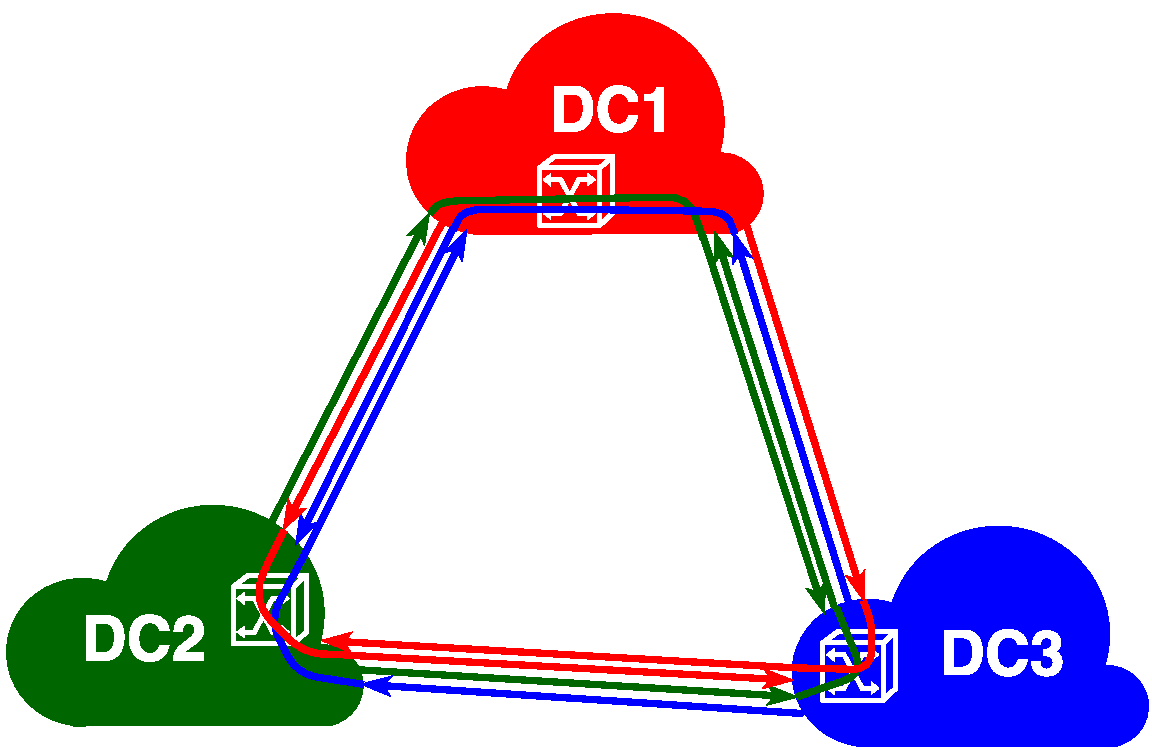
\includegraphics[width=0.48\textwidth]{images/inter-DC.pdf}
\caption{Partition an inter-DC network to multiple shards. Each color indicates a shard composed of one DC and the virtual routing paths originating from the DC.}
\label{fig:inter-dc}
\end{figure}



Intra-datacenter (intra-DC) routing paths are typically loop-free (Sec.~\ref{sec:dcn}), leading to efficient hierarchical aggregation. However, inter-DC routing paths are typically not loop-free. Fortunately, there is typically no ``hairpin'' traffic in inter-DC routing tables: packets passing through DC $A$ will never pass through some other DC $B$ and come back to $A$.

We partition the inter-DC network to $N$ logical shards, where $N$ is the number of DCs. Each shard is composed of one unique DC and all inter-DC traffic originating from the DC. Therefore, each inter-DC link is logically split to $N$ logical links, each carrying traffic originating from one DC.
The partitioning can be implemented by tagging each packet with an origin DC ID.
In this way, each switch in inter-DC WAN is logically split into $N$ switches, and at most $N$ beacon messages per inter-DC link are needed in each beacon interval.
Because the routes in each shard originate from a same DC, they form a DAG and are loop-free by our definition.\RED{(confused, loop-free logical shard leads to what?)}
Note that loop-free only affects liveness and is not required by correctness, therefore temporary routing loops will only stall message delivery until the loop disappears.

Typically, transit traffic of a DC only goes through border switches, analogous to ``international zones'' in an airport. If this is the case, we can handle intra-DC traffic as if no other DCs are present. For an incoming packet from another DC, the border switch removes the origin DC tag; for an outgoing packet, the border switch adds the origin DC tag.
\fi
